\section{Aufbau}\label{sec:aufbau}
\begin{center}
    \makebox[\textwidth][c]{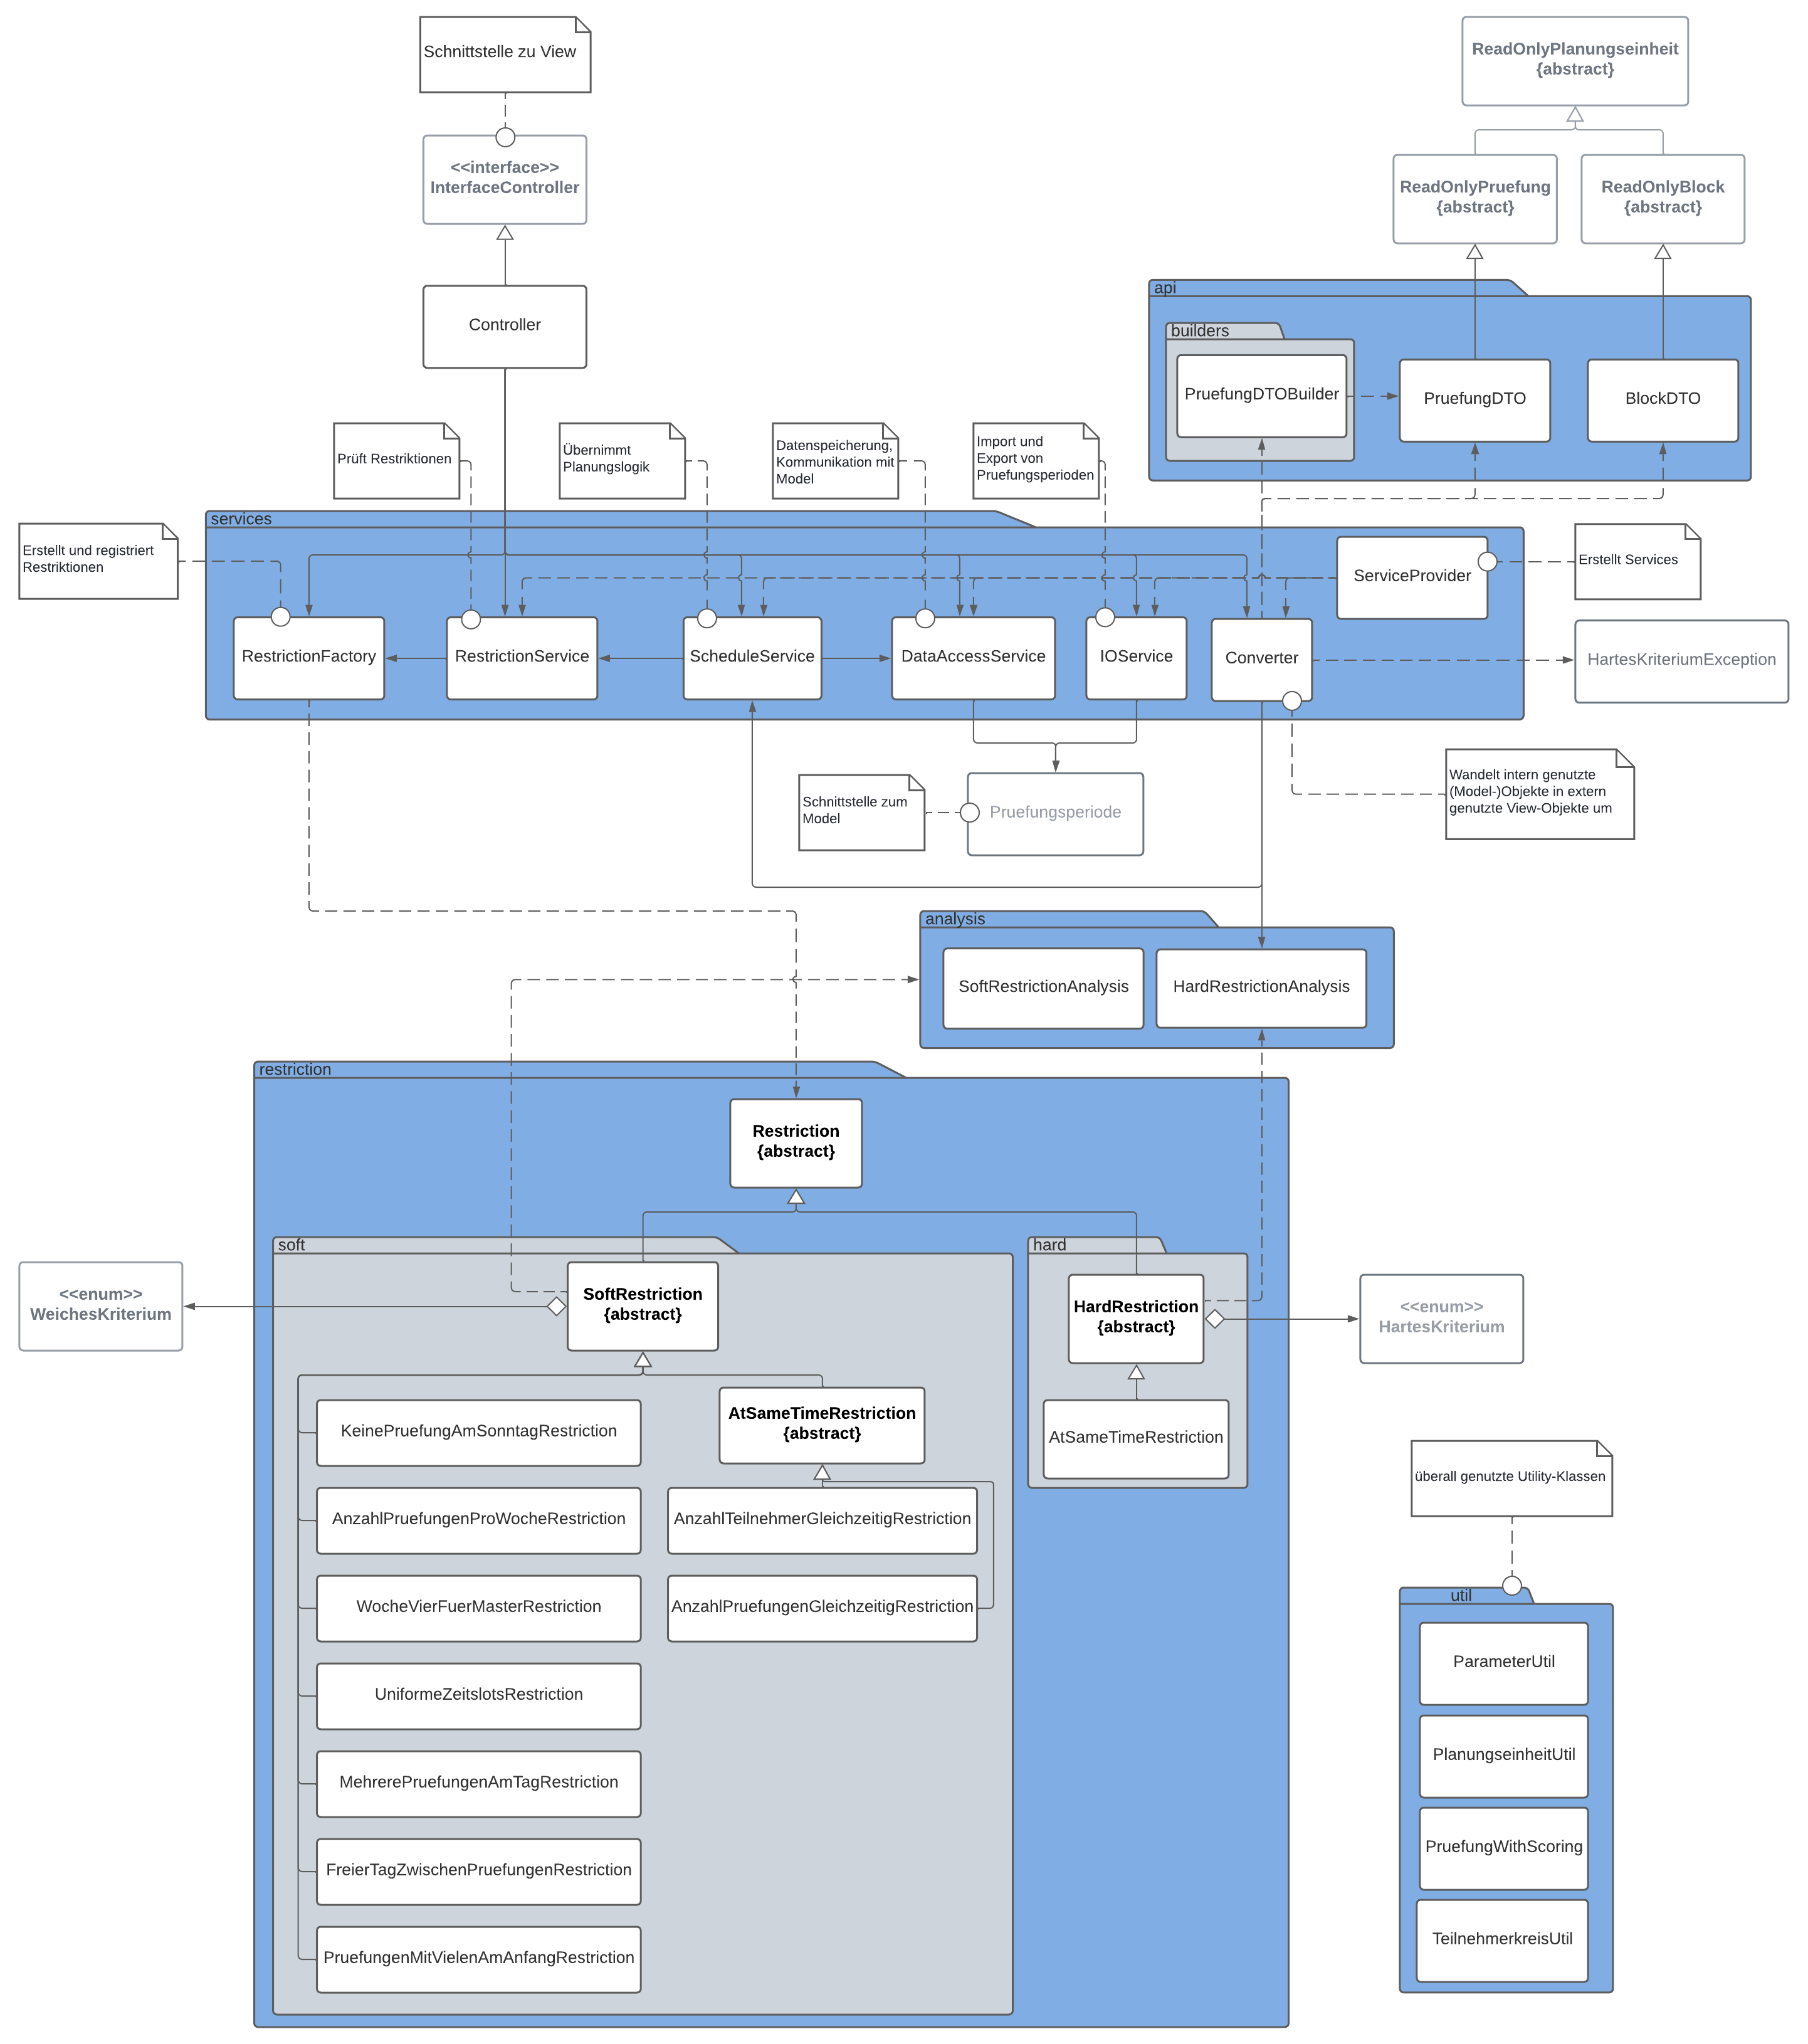
\includegraphics[width=1.25\textwidth]{extra/controller_2_uml}}%
\end{center}

\clearpage
Den Einstieg des Projekts von View-Seite bildet die Klasse \enquote{Controller}.
Das Projekt selbst gliedert sich in fünf Haupt-Pakete, wobei sich die Hauptfunktionalität
auf die Pakete \enquote{services} und \enquote{restriction} beschränkt.

Die einzelnen Services dienen der logischen Trennung der im Controller angebotenen Funktionalität.
Während der \nameref{subsec:dataaccessservice} sich beispielsweise auf die Kommunikation mit dem Model fokussiert,
werden im \nameref{subsec:ScheduleService} alle Planungen vorgenommen.
Genauere Beschreibungen zu den Services finden sich im Abschnitt \nameref{sec:Services}.
Das Package \enquote{restriction} beinhalten alle Restriktionen, die für das Planen von Prüfungen
und Blöcken ausgewertet werden (siehe \nameref{sec:restrictions}).

Neben dem Paket \enquote{util}, welches Hilfsklassen beinhaltet, gibt es außerdem das Package \enquote{api}
in dem sich Implementierungen der ReadOnly-Klassen finden, die für die Kommunikation mit View dienen
und das Package~\enquote{analysis}, das Klassen zur internen Kommunikation von Restriktions-Auswertungen enthält.

